\documentclass[12pt]{article}
\usepackage{fullpage}
\usepackage{amsmath, amsthm, amssymb}
\usepackage{enumerate}
\usepackage{mathtools}
\usepackage{multicol}
\usepackage{nicefrac}
\usepackage{graphicx}
\usepackage{hyperref}

\usepackage{tikz}
\usetikzlibrary{calc}
\usetikzlibrary{backgrounds}
\usepgflibrary{shapes}
\usetikzlibrary{through}

\usepackage{float}
\newtheorem{lemma}{Lemma}
\newtheorem{theorem}{Theorem}
\newtheorem{claim}{claim}
\newtheorem*{lemma*}{Lemma}
\newtheorem*{theorem*}{Theorem}
\newtheorem*{claim*}{Claim}
\usepackage{subcaption}

\newcommand*{\Real}{\mathbb{R}}
\newcommand*{\Z}{\mathbb{Z}}
\newcommand*{\Q}{\mathbb{Q}}
\newcommand*{\F}{\mathbb{F}}
\newcommand*{\ord}{\mathrm{ord}}
\newcommand*{\nil}{\mathfrak{N}}
\newcommand*{\inv}{^{-1}}

\begin{document}

\title{MATH 4320 Homework 5}
\author{Dominick Twitty}
\date{}
\maketitle

\section{On Algebraic Elements of an Extension}
%TODO 1
\begin{claim*}
Let $F$ be a field and $K$ be an extension. If $\alpha, \beta \in K$ are algebraic, then $\alpha \pm \beta$, $\alpha \beta$ and $\nicefrac{\alpha}{\beta}$ are also algebraic.
\end{claim*}
\begin{proof}
Let $\alpha$ be a root of $a$ and $\beta$ a root of $b$ with $a, b \in F[x]$. Then
\begin{align*}
\sum_{j = 0}^n a _ j \alpha ^ j = 0 && \text{and} && \sum_{k = 0}^m b _ k \beta ^ k = 0
\end{align*}


\noindent 
\end{proof}



\section{On Nilpotents and Ideals}
\begin{claim*}
$\nil(R)$ is ideal in $R$.
\end{claim*}
\begin{proof}
First, we show that $\nil(R)$ is a group under addition. Clearly, $0$ is in $\nil(R)$. Next, for some $x,y \in R$, let $x^n = y^m = 0$. We see
\[ (x + y) ^ {m + n - 1} = \sum_{k = 0}^{m + n - 1} \binom{n}{k} x^{m + n - 1 - k} y^k = 0\]
Finally, let $x ^ m = 0$. If $m$ is even, then $(-x) ^ m = x ^ m = 0$. If $m$ is odd, then $(-x) ^ {m + 1} = (-x)(-x)^m = 0$. Then $\nil(R)$ is a group under addition. Next, we must show that $\nil(R)$ absorbs multiplications. Let $x^m = 0$, and $y \in R$. Then
\[ (xy) ^ m = x^m y^m = 0 \]
So, $\nil(R)$ is an ideal. An alternative proof is that $\nil(R) = \sqrt{\{0_R\}}$. We see that $\{0_R\}$ is an ideal, and we showed in a previous homework that radical of an ideal is an ideal.
\end{proof}

\begin{claim*}
$R/\nil(R)$ has only $0$ as a nilpotent element.
\end{claim*}
\begin{proof}
Let $(x + \nil(R)) ^ m = (0 + \nil(R))$. Then 
\[(x + \nil(R))^m = (x ^ m + \nil(R)) = 0 + \nil(R)\]
So, $x^m \in \nil(R)$, then $x \in \nil(R)$. So, $(x + \nil(R)) = (0 + \nil(R))$. 
\end{proof}


\section{On Polynomial Quotient Fields}
Let $f = x^2  + x + 1 \in \F_2[x]$. Let $I = (f)$, and $E = \F_2[x] / I$. By Theorem 3.115 in the textbook, we can say that every $e \in E$ has a unique expression of the form $a + b(x + I)$ where $a,b \in \F_2$ and $(x + I)$ is a root of $f$. There are four choices of $(a, b)$, so $E = \{0 + I, 1, x + I, 1 + x + I\}$. As shown in the proof of Theorem 3.115, by the division algorithm, if $g = qf + r$, then $g + I = r + I$. This gives us the following three equations
\begin{align*}
(x)(x) = x^2 = f + x + 1 &\implies (x + I)(x + I) = (x + 1 + I)\\
(x)(x + 1) = x^2 + x = f + 1 &\implies (x + I)(x + 1 + I) = (1 + I)\\
(x + 1)(x + 1) = x^2 + 1 = f + x &\implies (x + 1 + I)(x + 1 + I) = (x + I)
\end{align*}
\noindent and the multiplication table
\[
\begin{array}{c | c c c c}
      & \,\,0\,\, & \,\,1\,\, & \,\,x\,\, & x + 1\\\hline
0     & 0 & 0     & 0     & 0\\
1     & 0 & 1     & x     & x + 1\\
x     & 0 & x     & x + 1 & 1\\
x + 1 & 0 & x + 1 & 1     & x
\end{array}
\]
Every nonzero element of $E$ has an inverse, then $E$ is a field, then $f$ is irreducible.

\section{On $x^3 - 2x - 2$ in $\Q[x]$}
Let $f = x^3 - 2x - 2 \in \Q[x]$. We see that $f$ meets the Eisenstein Criterion with prime $p = 2$, and is therefore irreducible over $\Q$. Let $\theta$ be a root of $f$. We see that 
\begin{align*}
(3 + \theta)(5 \theta^2 -2\theta + 10) &= 5\theta^3 + 13 \theta^2 + 4\theta + 30\\
&= 5f(\theta) + 13\theta^2 + 14\theta + 40\\
&= 13\theta^2 + 14\theta + 40
\end{align*}

Let $g = 5\theta^2 - 2\theta + 10$. We wish to find some $h$ such that $hg = 1 \equiv qf + 1$. Given that $f$ and $g$ are relatively prime ($f$ is irreducible and does not divide $g$), we can find $h$ and $q$ using the Extended Euclidean Algorithm. With the help of a computer algebra system, we find that $\frac{1}{h} = g$ with
\begin{align*}
g = \frac{-96 \theta^2 + 70\theta + 412}{5204} 
&& \text{and} && 
gh = \left(\frac{-120\theta}{1301} + \frac{271}{2602}\right)f + 1
\end{align*}
\section{}
%TODO 5
\section{}
%TODO 6
\section{}
%TODO 7


\section{Inscribing a Hexagon in a Circle}
Consider some regular hexagon $H$ inscribed in a circle $C$ with center $o$ and radius $r$. Let $p_1$ and $p_2$ be adjacent vertices of $H$. We see that the triangle $(p_1,p_2,o)$ is equilateral. From this, we can say that the side length of $H$ is exactly equal to $r$.

\begin{figure}[H] \centering
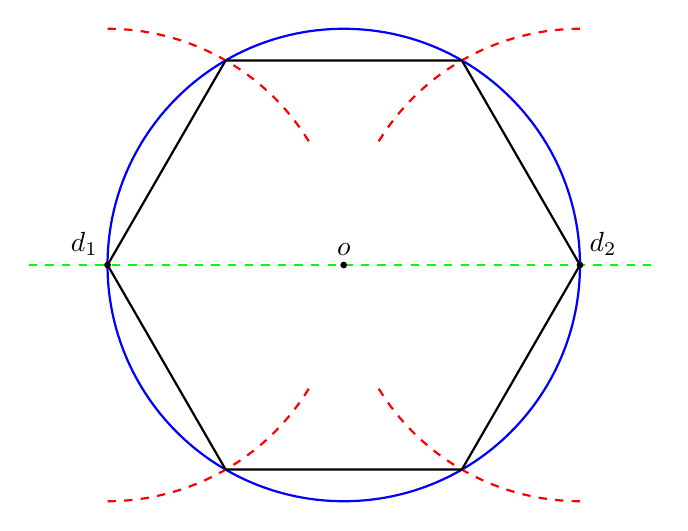
\begin{tikzpicture}
    % the circle
    \draw[thick, blue] (6*2,0) circle(3cm);
    
    % the center line
    \draw[thick,green,dashed] (8,0) -- (16,0);
    
    % the arcs from d1 and d2
    \draw[thick,red,dashed] (9,3) arc (90:30:3);
    \draw[thick,red,dashed] (9,-3) arc (-90:-30:3);
    \draw[thick,red,dashed] (15,3) arc (90:150:3);
    \draw[thick,red,dashed] (15,-3) arc (-90:-150:3);
    
    % the constructed hexagon
    \node[thick, regular polygon, regular polygon sides=6, minimum size=6cm, draw] at (6*2,0) {};
    
    % labelled points
    \draw [fill=black] (12,0) circle (1pt);
    \node[above] at (12,0) {$o$};
    \draw [fill=black] (9,0) circle (1pt);
    \node[above left] at (9,0) {$d_1$};
    \draw [fill=black] (15,0) circle (1pt);
    \node[above right] at (15,0) {$d_2$};
\end{tikzpicture}
\end{figure}

This gives us an easy way to construct $H$, which we illustrate above. Draw a line (shown in green) across $C$, passing through $o$, to find points $d_1$ and $d_2$ exactly opposite each other on $C$. Set the radius of the compass to $r$ by extending it from $d_1$ to $c$. Intersect arcs (shown in red) of radius $r$ centered at $d_1$ with $C$, and do the same with $d_2$. Connect the six points to draw an regular inscribed hexagon.

By construction, each intersection point is distance $r$ from its arc center. We know $d_1$ and $d_2$ can be part of a hexagon, as they are exactly opposite each other. We showed above that the points of distance $r$ away from $d_1$ on $C$ must also be part of the hexagon, so the four intersections are also part of the hexagon. 

\section{}
%TODO 9
\section{}
%TODO 10

\end{document}
